% File: 03-tail/01_appendix_example.tex
\chapter{Distribution by rater}
\label{app:distribution}
\minitoc
\begin{figure}[htbp]
    \centering

    % First figure
    \begin{subfigure}[b]{0.7\textwidth} % Adjust width for single column
        \centering
        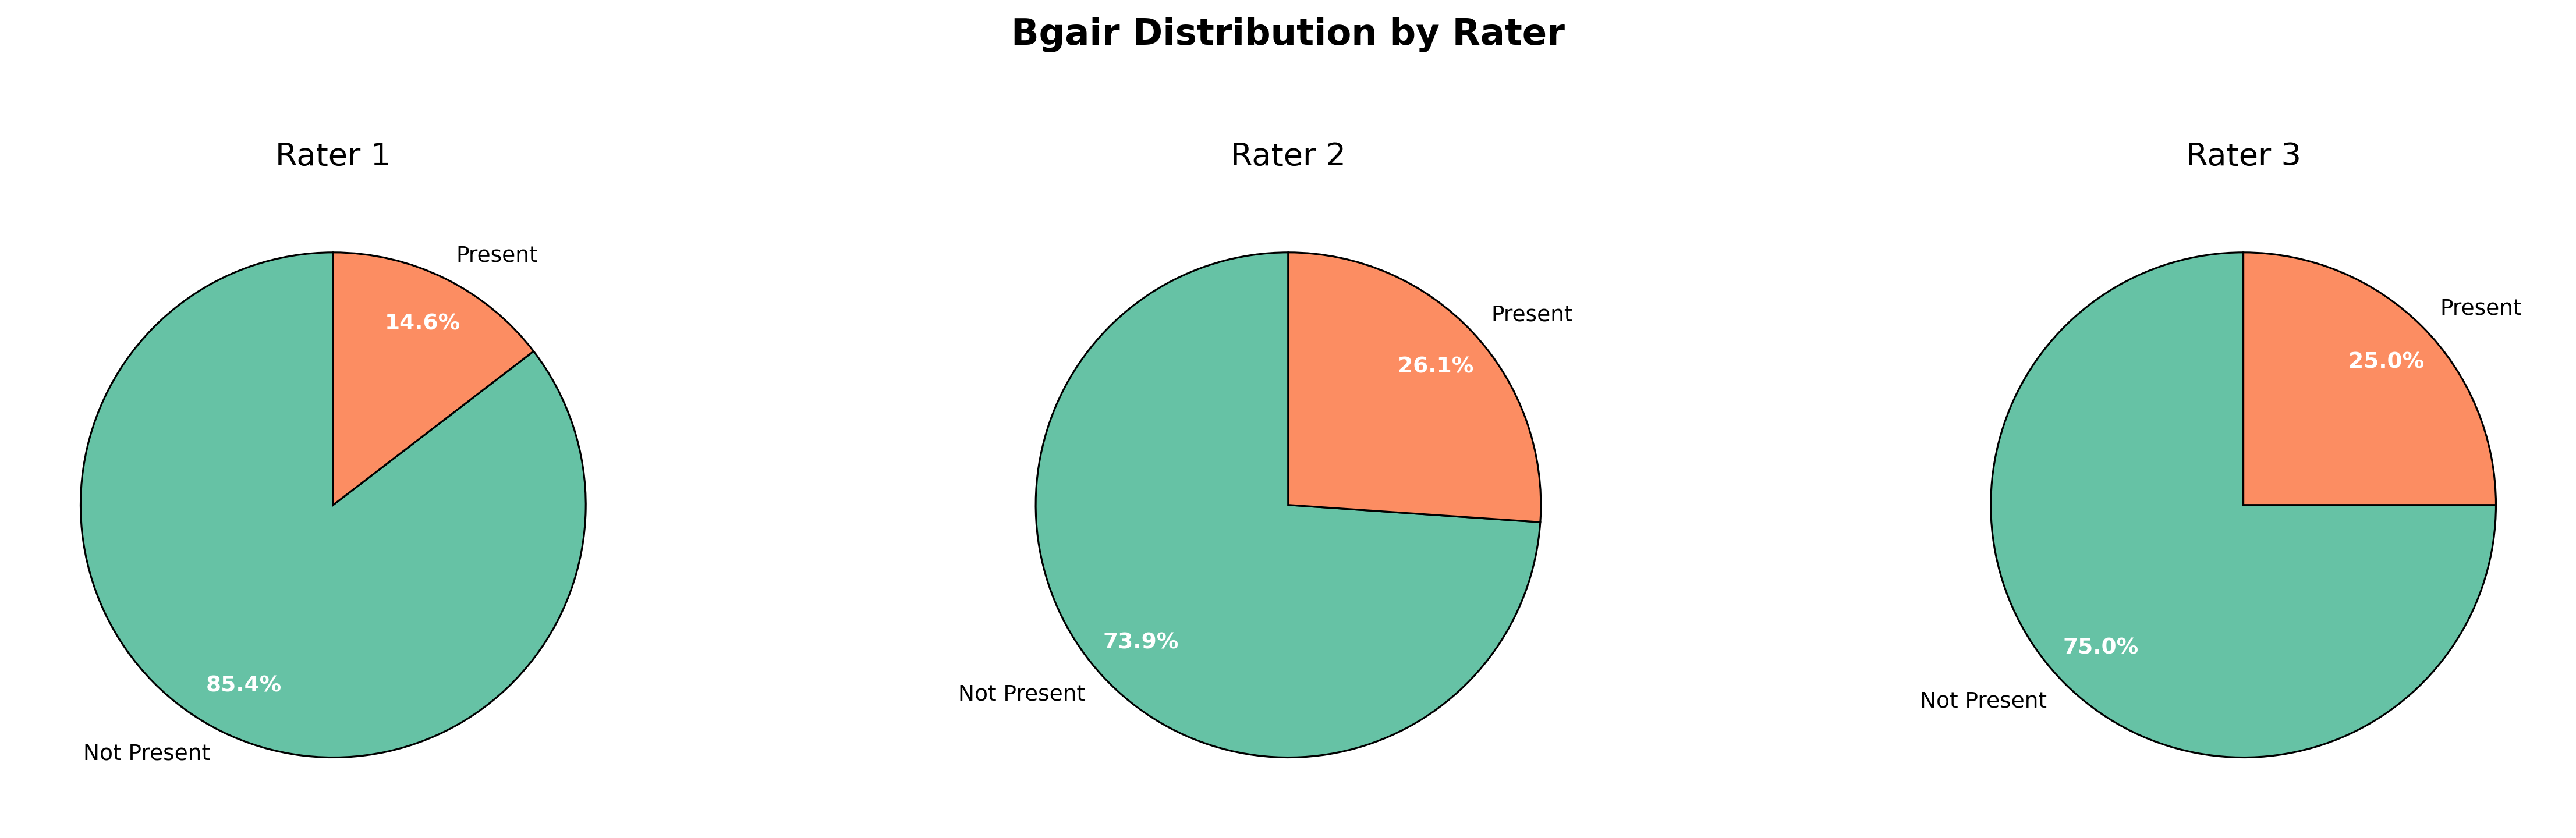
\includegraphics[width=\linewidth]{Report/img/bgair_by_rater_pie.png}
        \label{subfig:bgair_distribution_single} % Unique label for this subfigure
    \end{subfigure}

    \vspace{4mm} % Add vertical space between figures

    % Second figure
    \begin{subfigure}[b]{0.7\textwidth} % Adjust width for single column
        \centering
        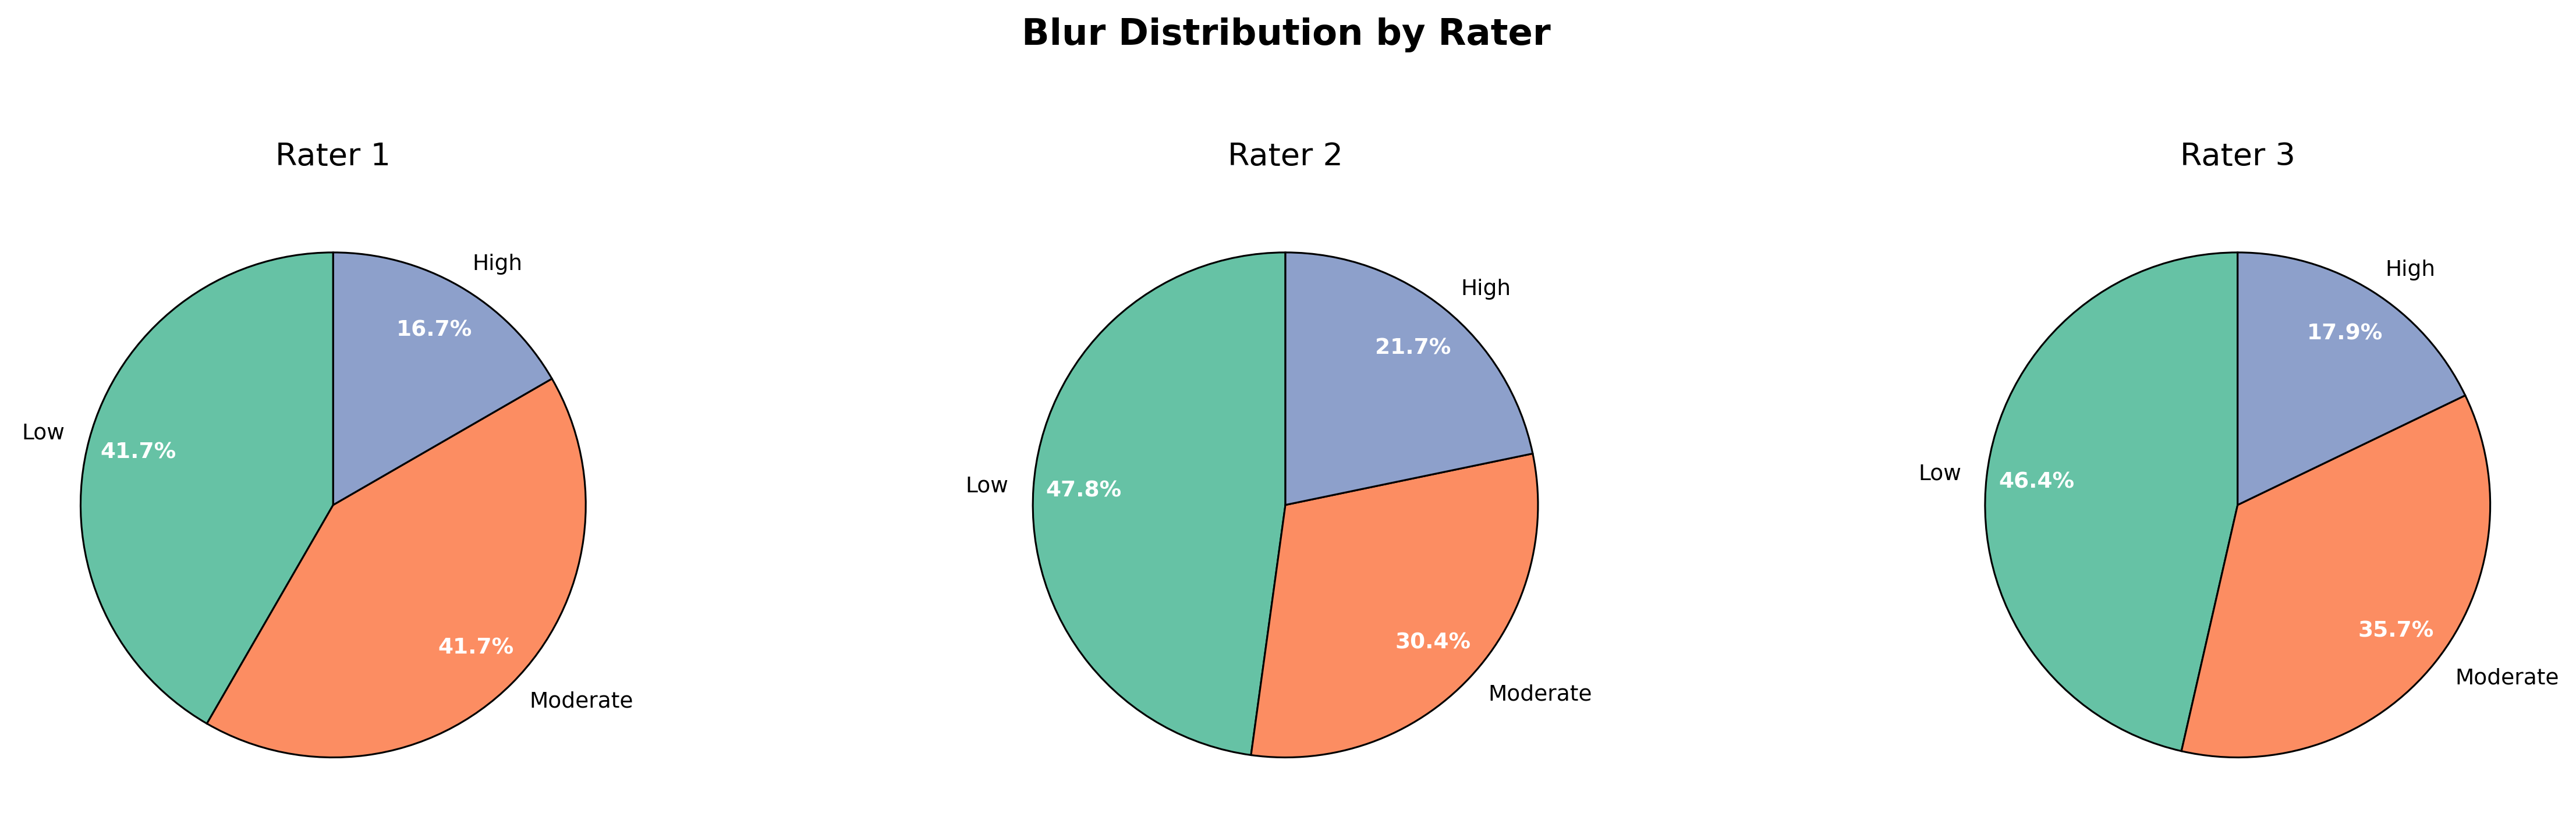
\includegraphics[width=\linewidth]{Report/img/blur_by_rater_pie.png}
        \label{subfig:blur_distribution_single}
    \end{subfigure}

    \vspace{4mm} % Add vertical space between figures

    % Third figure
    \begin{subfigure}[b]{0.7\textwidth} % Adjust width for single column
        \centering
        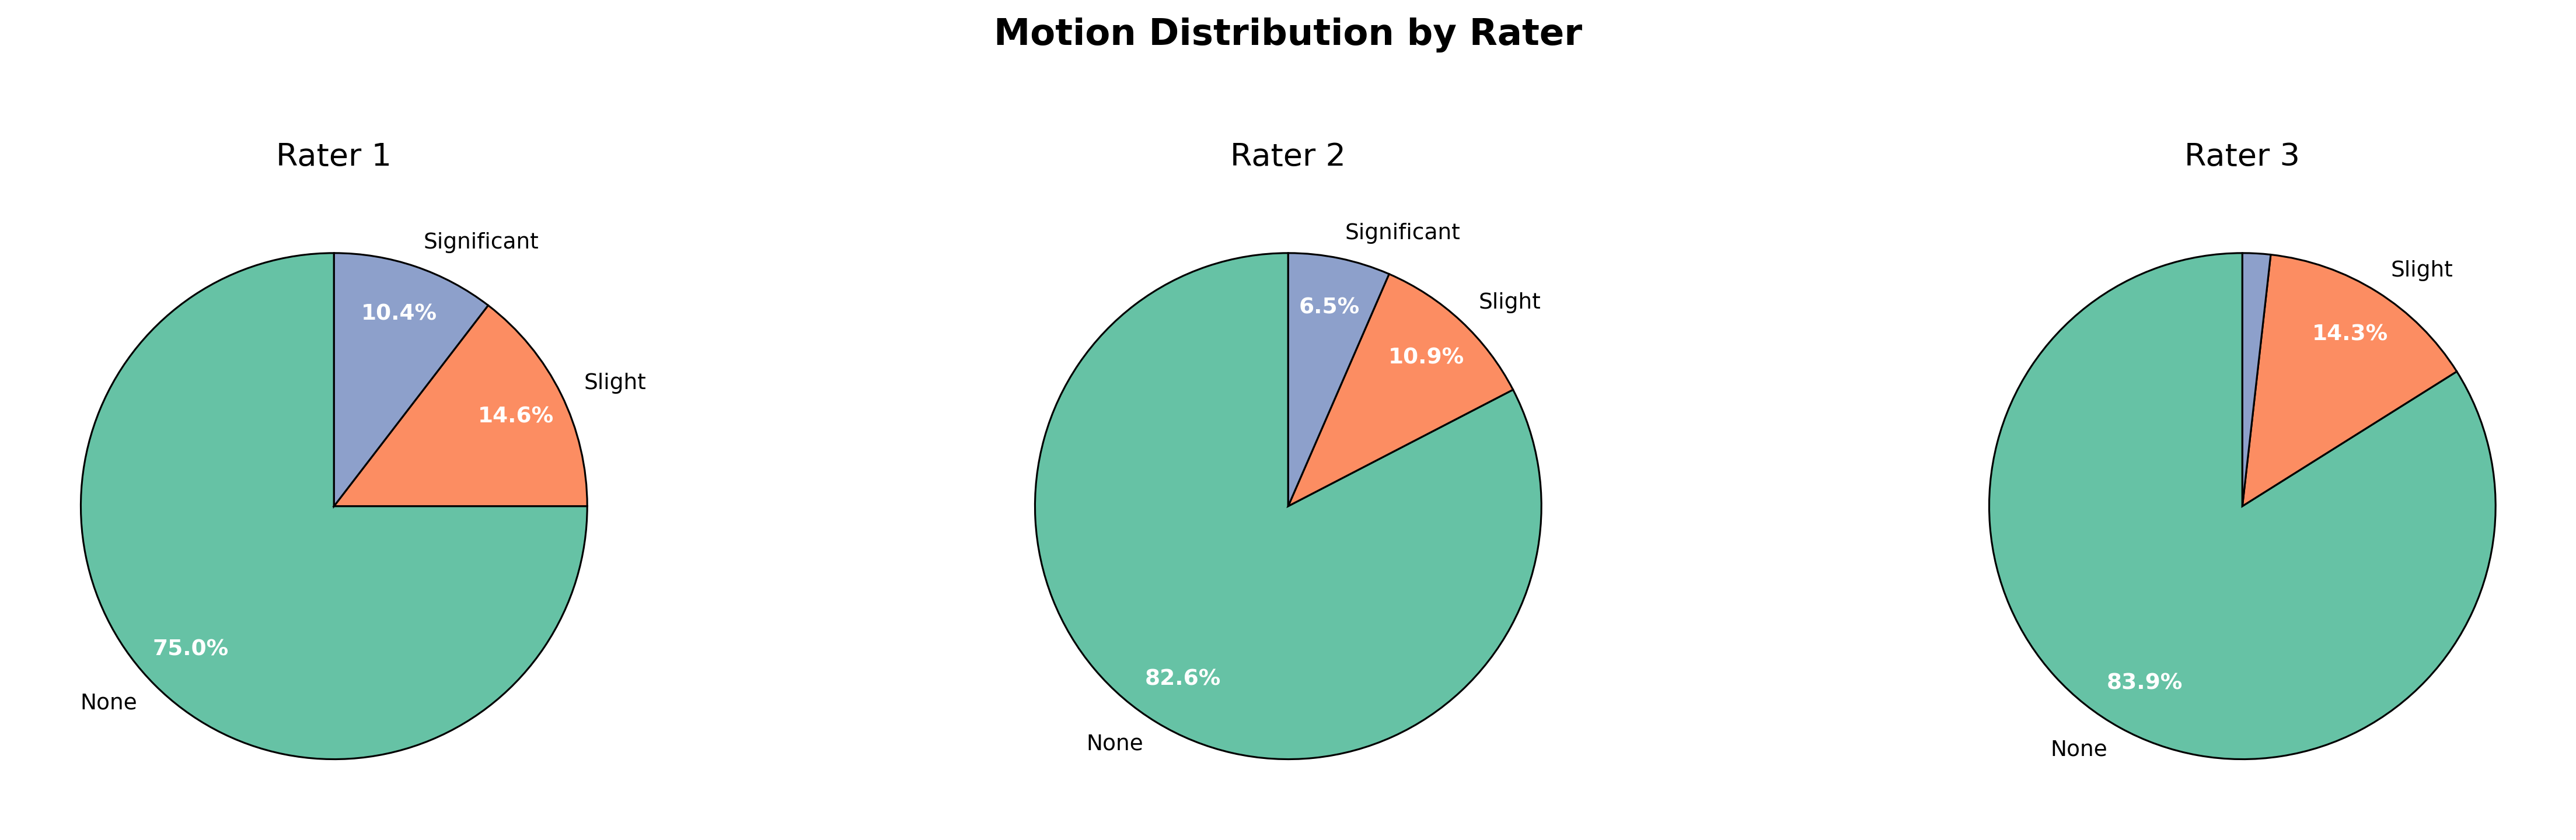
\includegraphics[width=\linewidth]{Report/img/motion_by_rater_pie.png}
        \label{subfig:motion_distribution_single}
    \end{subfigure}

    \vspace{4mm} % Add vertical space between figures

    % Fourth figure
    \begin{subfigure}[b]{0.7\textwidth} % Adjust width for single column
        \centering
        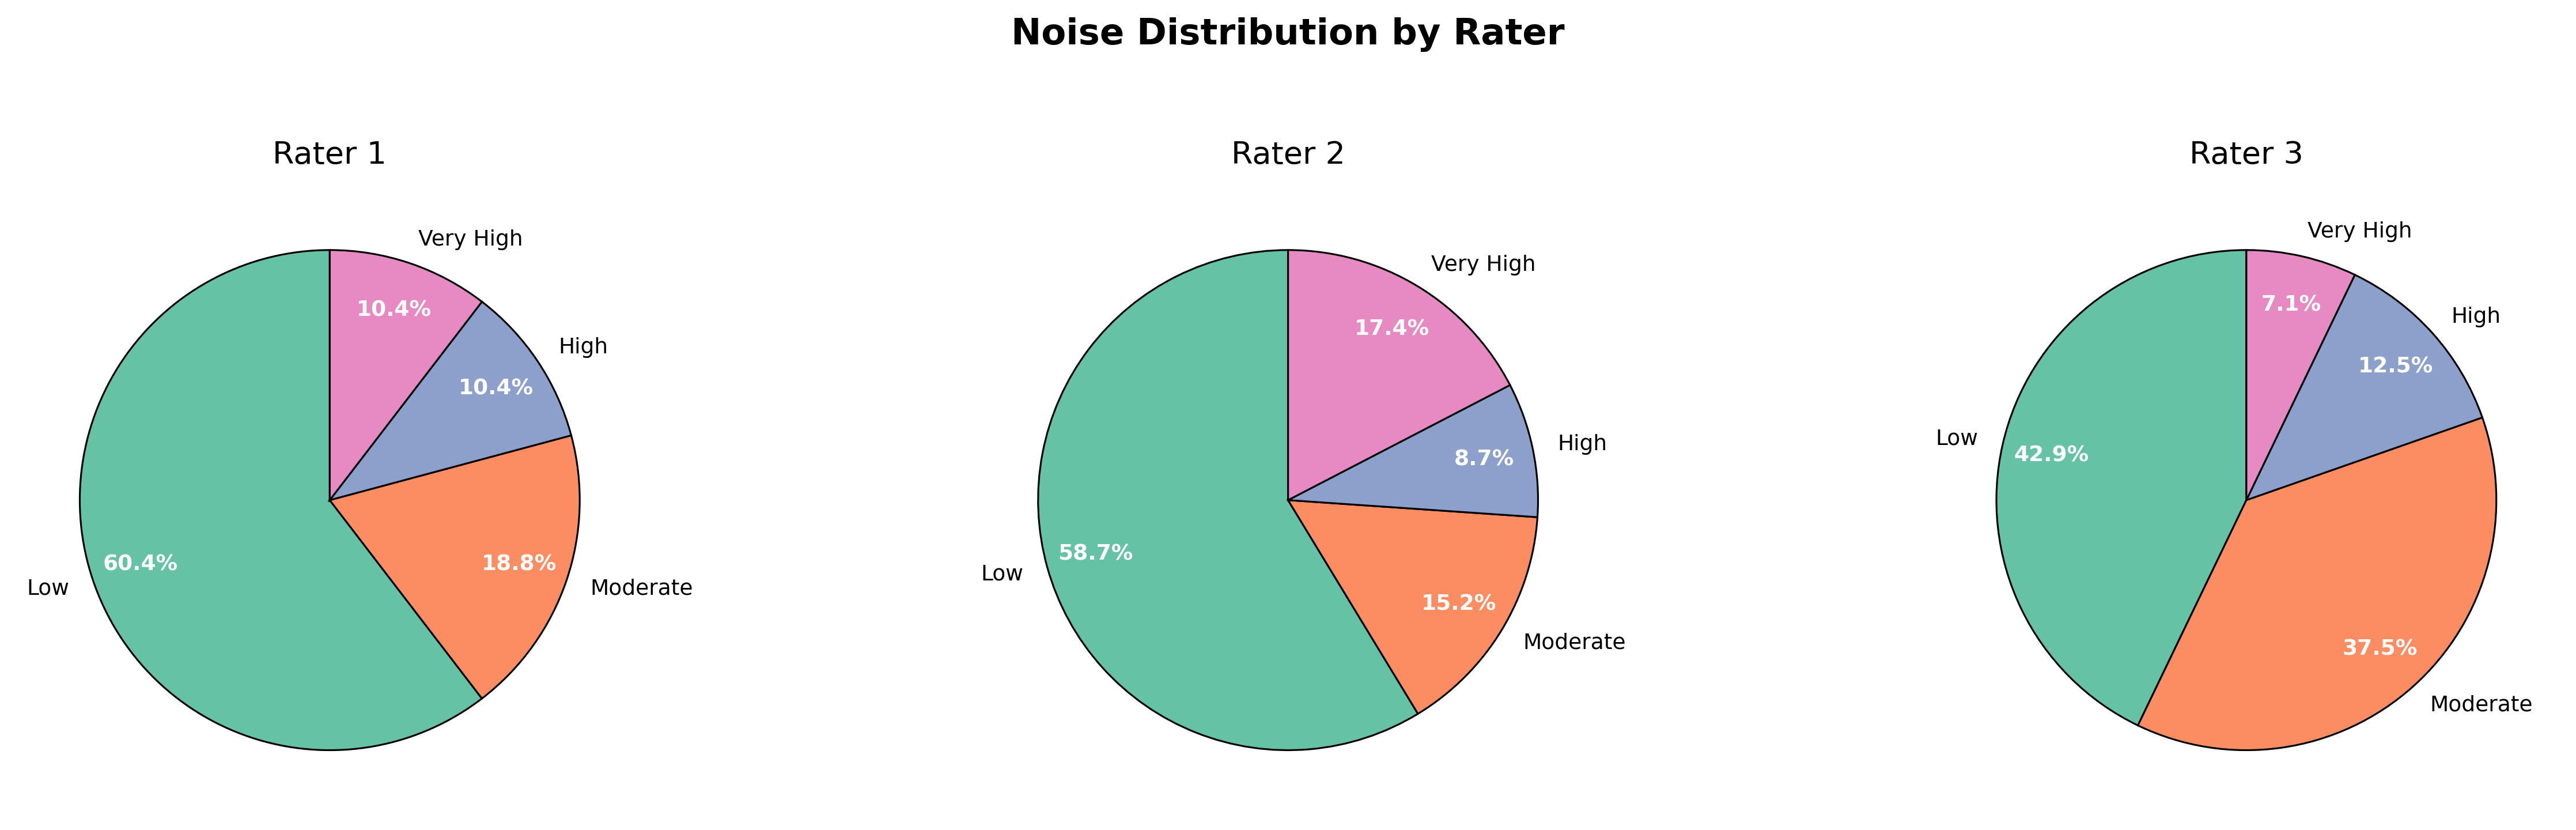
\includegraphics[width=\linewidth]{Report/img/noise_by_rater_pie.png}
        \label{subfig:noise_distribution_single}
    \end{subfigure}

    \caption{Distribution of artifact severity ratings by rater across different categories: (a) Background Artifacts (Bgair), (b) Blur, (c) Motion, and (d) Noise. These pie charts illustrate variations in how frequently each rater assigned images to the various quality categories for each specific artifact.}
    \label{fig:artifact_distributions_by_rater_single_column} % Overall label for the figure
\end{figure}